\documentclass{report}
\usepackage[T1]{fontenc}
\usepackage[utf8]{inputenc}
\usepackage[english]{babel}
\usepackage{graphicx}
\usepackage{fancyhdr}
\pagestyle{fancy}
\lhead{\textbf{System and device programming}}
\rhead{Laboratory 5}
\lfoot{Enrico Franco}
\rfoot{Politecnico di Torino}
\author{Enrico Franco}
\title{System and Device Programming \\
	Laboratory 5 - Exercise 1}
\begin{document}
\section*{Exercise 1}
\texttt{pack.sh}, stored in SDP/MK/, is a bash script which can work, with an appropriate dimension, with every kernel and also on a physical disk, even if, in this case, a \texttt{.img} file with a small kernel is generated. The script takes a single argument, representing the number of kilobytes to allocate for the partition and stores it in variable \texttt{kbytes}. This partition will contain a file system composed by GRUB and a kernel.

First, the script clears log files \texttt{pack1.txt} and \texttt{pack2.txt} and it sets properly user and group, \emph{laface} in this case. This is a necessary operation because the script must run with \emph{sudo privileges} and at the end of the procedure, it is needed to restore the user permissions.

With the instruction \texttt{dd} (disk dump), the script creates an output file \emph{hd.img}, with block size 512 bits (option \texttt{bs}) and size \texttt{kbytes*1024*512} bits, filled with zeros because input file is \emph{/dev/zero}. The option \texttt{count=1} means that a sector is skipped because it has to be filled with the master boot record. \texttt{losetup} sets \emph{hd.img}, which is a normal a file, as a device named \emph{/dev/loop1}. In this way it possible to use device commands, for example \texttt{fdisk}. Starting from here, \emph{hd.img} and \emph{/dev/loop1} are the same thing.

A file \texttt{fdisk.input} is created to infer instructions to the command \texttt{fdisk} interactively. This file is generated exploiting both input and output redirection of command \texttt{cat}. In fact, this command, which normally produces output on console, is redirected to file \texttt{fdisk.input} and input, which normally is given from the keyboard, is hard-written in \texttt{pack.sh} and it is taken by \texttt{cat} command until \texttt{EOF} is caught. Thus, characters are written onto file \texttt{fdisk.input}.

\begin{itemize}
\item First, exploiting \texttt{cat} redirection, enter in expert mode (\texttt{x}), set 16 heads (\texttt{h 16}) and 63 sectors (\texttt{s 63}).
\item In order to set the number of cylinders it is needed to use option \texttt{c} and append the content of \texttt{kbytes} to \texttt{fdisk.input} performing a \texttt{echo} properly redirected.
\item Then, exploiting \texttt{cat} redirection again, a new partition is created (\texttt{n}), numbered \texttt{1} and it is made bootable (\texttt{a}). Finally it is possible to write modification and exit (\texttt{w}). 
\end{itemize}

At this point, the way on which create partition is stored in \texttt{fdisk.input}. Therefore, it is possible to use command \texttt{fdisk}, which allows to create and manage partitions, on disk \emph{hd.img} (i.e.\@ the virtual hard disk the script is creating) and infer commands stored on file to create and set the disk.

Number of blocks is got through the command \texttt{fdisk -l -u}, which returns some lines containing various information of the disk and stored on variable \texttt{blocks} by properly elaborating the output of the command. In fact, only the last line is considered (\texttt{| tail}), blanks are removed (\texttt{| tr -s " "}), the ``column'' 5 is taken (\texttt{| cut -d " " -f 5}) and the character `+' in front of the number of blocks is removed (\texttt{| cut -d "+" -f 1}). 

\emph{/dev/loop1} is detached using option \texttt{-d} of command \texttt{losetup} from \emph{hd.img}. Since this operation takes some time, \emph{hd.img} is attached to a new device, \emph{/dev/loop0} this time, starting at offset \texttt{63*512} in order to leave some space for MBR\footnote{Master Boot Record} and its size as \texttt{blocks*1024} to avoid exceeding the virtual partition. Finally, an \emph{ext2} file system is created on \emph{/dev/loop0}, which corresponds to \emph{hd.img}, using command \texttt{mkfs.ext2}.

\medskip

Exploiting redirection of command \texttt{cat} it is possible to create a simple menu for the GRUB, stored in file \texttt{menu.lst}. This file contains the title, the information about the location of kernel (i.e.\@ \texttt{/boot/minimal\_linux\_kernel}) and root directory (i.e.\@ \texttt{dev/hda}) and some options indicating that it is read-only (\texttt{ro}), mount is quiet, i.e.\@ not verbose (\texttt{quiet}), and it has to show a splash window (\texttt{splash}) if it possible to choose more than one kernel on bootstrap. Statement \texttt{initrd} is not necessary in this case, because no file system inside the kernel has to be created. This option may be useful for other types of kernel.

A directory \texttt{mount\_point} is created inside the file system and it will be the mount point for the device \emph{/dev/loop0}. In this directory, subdirectories \texttt{boot/grub} are created and some GRUB and kernel files are copied. At this point, it is possible to umount the device, remove the directory (files has already been copied in the device, and hence in \emph{hd.img}) and detach \emph{/dev/loop0} from \emph{hd.img}.

Then, it is possible to create the \texttt{grub.input} file for GRUB, exploiting both input and output redirection of command \texttt{cat}. In this file it is needed to indicate that the device is on the first partition of \texttt{hd0}, named \texttt{hd.img}. Some geometry parameters are needed, such as number of kilobytes (variable \texttt{kbytes}), number of heads and sectors. Device \texttt{root} is added in \texttt{hd0} and GRUB is setup to start.

\medskip

Finally, \texttt{grub.input} file is given to \texttt{grub.bin} in order to copy those two stages of GRUB in \texttt{hd.img}, so that it can be bootable.

Since all the instructions were run in \emph{sudo}, i.e.\@ with superuser privileges, it is needed to perform some \texttt{chown} to properly set user and group.

\bigskip
For each command which may produce some output or information, \texttt{sdtout} and \texttt{stderr}, corresponding respectively to file descriptor 1 and 2 are redirected to files \texttt{pack1.txt} and \texttt{pack2.txt} respectively.

\newpage

In order to execute \emph{hd.img}, it is needed to start \texttt{qemu}.

\begin{figure}[hbtp]
\centering
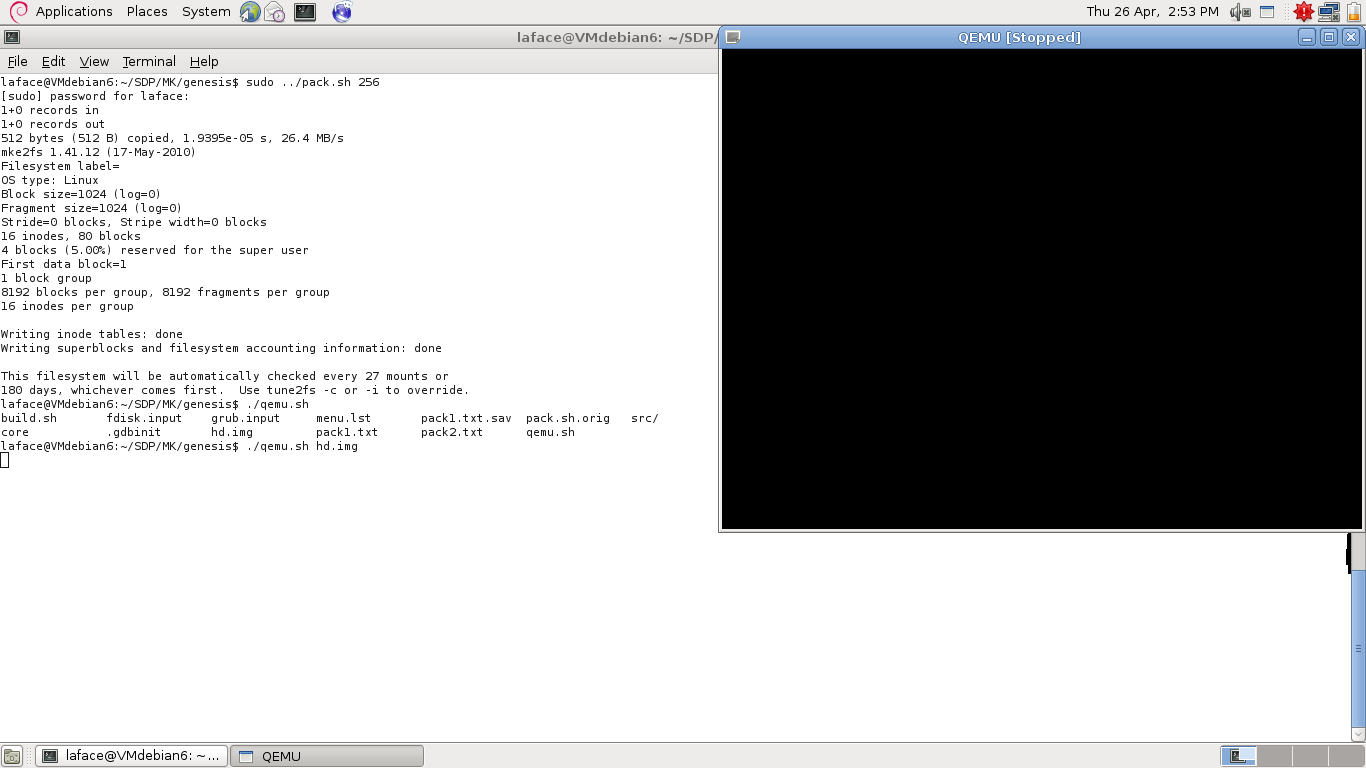
\includegraphics[scale=0.24]{images/es01/01_pack_qemu.png}
\caption{pack.sh result and qemu}
\end{figure}

Script \texttt{qemu.sh} receives as unique parameter, the \texttt{.img} file, it will start stopped (option \texttt{-S}) and it is possible to debug it exploiting gdb remotly on TCP port 1234.

\begin{figure}[hbtp]
\centering
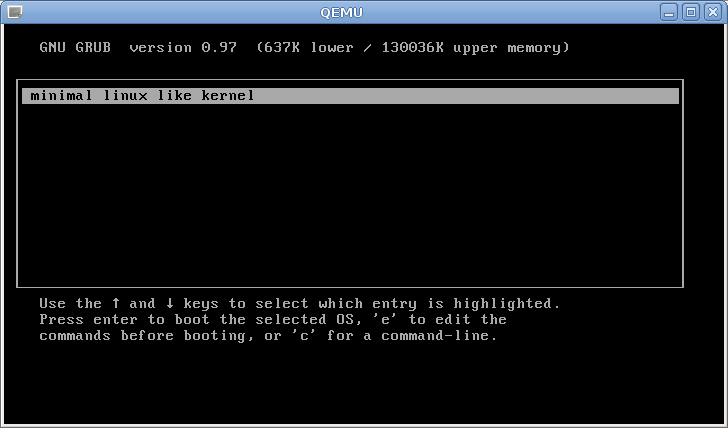
\includegraphics[scale=0.35]{images/es01/02_qemu_grub.png}
\caption{qemu showing GRUB}
\end{figure}

In order to debug the kernel, it is possible to exploit ddd, which is an improved graphical version of gdb, on target \emph{localhost:1234}\footnote{This information is contained in file \texttt{.gdbinit}}.

\texttt{0x7c50} represents the address where the GRUB begins, it is possible to set a break point through the gdb command \texttt{b *0x7c50} and debug the GRUB code.
\end{document}